\section{System Architecture}
\label{sec:system_architecture}

The system architecture of our AI-powered mobile application is designed to ensure modularity, scalability, and secure data handling. It is composed of three main components: the mobile application, the backend services, and the AI inference engine. Each component plays a distinct role while communicating seamlessly with the others.

The architecture follows a modular pattern to facilitate independent development and testing of each module. This design choice improves maintainability and simplifies the integration of additional features in the future.

The overall system structure is illustrated in Figure~\ref{fig:system-architecture}, which outlines the interactions between the core components of the application.


\begin{figure}[H]
    \centering
    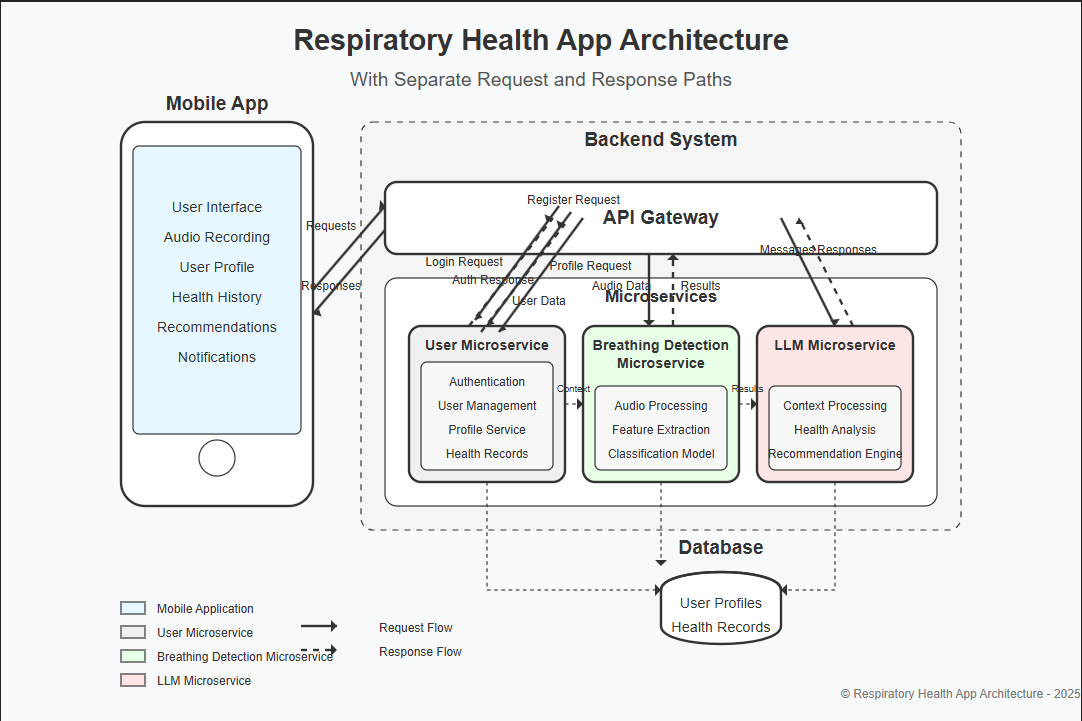
\includegraphics[width=\textwidth]{images/architecture.png}
    \caption{System Architecture of the AI-Powered Mobile Application}
    \label{fig:system-architecture}
\end{figure}

\subsubsection*{Mobile Application}

The mobile application, developed using Flutter, provides the user interface and handles client-side functionalities. These include audio recording, local encryption, file selection, and UI interactions. It also manages authentication and communication with the backend.

\subsubsection*{Backend Services}

The backend is powered by Appwrite, a self-hosted backend-as-a-service platform. It handles authentication, file storage (medical reports and audio), and serverless functions. Appwrite ensures secure and scalable data management while offering APIs that are easy to integrate with Flutter.

\subsubsection*{AI Inference Engine}

The AI inference module is responsible for analyzing respiratory audio data and generating preliminary diagnostic feedback. Once an audio file is uploaded and validated, it is sent to a dedicated inference server or function that runs a pre-trained deep learning model to detect anomalies in the breathing pattern.

\vspace{1em}

This modular architecture enables efficient development, enhances security, and supports the core functionality of respiratory disease detection.
